% TEMPLATE for Usenix papers, specifically to meet requirements of
%  USENIX '05
% originally a template for producing IEEE-format articles using LaTeX.
%   written by Matthew Ward, CS Department, Worcester Polytechnic Institute.
% adapted by David Beazley for his excellent SWIG paper in Proceedings,
%   Tcl 96
% turned into a smartass generic template by De Clarke, with thanks to
%   both the above pioneers
% use at your own risk.  Complaints to /dev/null.
% make it two column with no page numbering, default is 10 point

% Munged by Fred Douglis <douglis@research.att.com> 10/97 to separate
% the .sty file from the LaTeX source template, so that people can
% more easily include the .sty file into an existing document.  Also
% changed to more closely follow the style guidelines as represented
% by the Word sample file. 

% Note that since 2010, USENIX does not require endnotes. If you want
% foot of page notes, don't include the endnotes package in the 
% usepackage command, below.


\documentclass[letterpaper,twocolumn,10pt]{article}
\usepackage{usenix,epsfig,endnotes}
\usepackage{enumitem}
\usepackage{graphicx}
\usepackage{subcaption}
\usepackage{listings}
\usepackage{xcolor}


\renewcommand{\enoteheading}{%
  \section*{Notes}
  \vspace{-0.5em}
}

\definecolor{termcmd}{RGB}{0,80,180}
\definecolor{termbg}{RGB}{248,248,248}
\definecolor{termerr}{RGB}{160,30,30}
\definecolor{termok}{RGB}{20,110,40}
\definecolor{termgray}{RGB}{90,90,90}

\lstdefinestyle{terminal}{
basicstyle=\ttfamily\scriptsize,
breaklines=true,
frame=tb,
framerule=0.4pt,
rulecolor=\color{gray!50},
backgroundcolor=\color{termbg},
xleftmargin=6pt,
xrightmargin=6pt,
columns=flexible,
keepspaces=true,
showstringspaces=false,
aboveskip=3pt,
belowskip=3pt,
moredelim=[il][\color{termcmd}\bfseries]{\$ },
moredelim=[il][\color{termerr}\bfseries]{ERROR},
moredelim=[il][\color{termok}]{[+]},
moredelim=[il][\color{termgray}]{[*]},
}


\begin{document}
%don't want date printed
\date{}

%make title bold and 14 pt font (Latex default is non-bold, 16 pt)
\title{\Large \bf CS-412 Lab 2: Fuzzing Lib-PNG }

\author{
{\rm Wajiha Masood}\\
\and
{\rm Nicolas Sozzi}\\
\and
{\rm Sara Bosi}\\
\and
{\rm Adrian Martinez}
}

\maketitle

% Use the following at camera-ready time to suppress page numbers.
% Comment it out when you first submit the paper for review.
\thispagestyle{empty}

\section*{Introduction}
Fuzzing is a widely used technique for discovering vulnerabilities in software by automatically generating and mutating inputs to trigger unexpected behavior. In this lab, we apply coverage-guided fuzzing to libpng 1.4.8, a widely deployed open-source library for decoding and encoding PNG images, using AFL++. Given that libpng is embedded in browsers, image editors, and countless other applications, memory corruption bugs in its parsing logic can have significant real-world impact. We describe the design of our fuzzing harness, our instrumentation choices, seed corpus construction, and the analysis of crashes discovered during the campaign, including a heap-based out-of-bounds read in the iTXt chunk parser.

\section {Harness Design}
We selected \texttt{png\_read\_info()}, \texttt{png\_read\_image()} along with the progressive parser using the
\texttt{png\_process\_data()} API as the main entries in the harness. Such APIs make great targets for fuzzing since they are responsible for parsing the user-supplied PNG file and involve complicated operations like handling the chunks in the image, parsing, decompressing the image contents, transforming color values and allocating memory dynamically. The decoders are traditionally one of the main culprits when it comes to memory corruption bugs since the binary format could easily cause an out-of-bounds access, integer overflows or heap corruption.
\subsection{Alternative Entry Points}
We also explored Libpng write/encoder APIs such as \texttt{png\_write\_image()} and other write APIs,  but fuzzing the decoder API was found to be more promising as decoding involves working with user-generated PNG files, whereas encoding works with image data generated by applications. Fuzzing the decoder revealed much more interesting behavior than fuzzing the write API; no crashes were encountered when fuzzing the latter. Thus, the decoder APIs were chosen as the main target for fuzzing.
\subsection{Harness Data flow}
The workflow for the harness starts with AFL++ generating a mutated PNG input and passing it to the harness. The input file is then read into a memory buffer that is modeled as a struct that contains data pointers to the input, total size and current offset. With a customized callback function passed to \texttt{png\_set\_read\_fn()}, libpng will be able to read directly from the AFL++ controlled buffer instead of from a regular file stream. Through repeated callbacks during execution, libpng will keep requesting bytes, which results in the AFL++ mutated input being sent to the parser. The typical harness involves initializing structures in libpng, reading the PNG header information with \texttt{png\_read\_info()}, reading metadata from the header using \texttt{png\_get\_IHDR()}, activating multiple transform functions, allocating buffers for rows, decoding the PNG images with \texttt{png\_read\_image()}, and lastly parsing additional chunks with \texttt{png\_read\_end()}.

\subsection{Guard Rationale}

Several guards were included to increase fuzzing robustness and ensure that all crashes occur only because of libpng code rather than harness itself. Checks for null after function calls \texttt{png\_create\_read\_struct()} and \texttt{png\_create\_info\_struct()} ensure that crashes are not occurring trivially due to failed allocations. It's crucial to include the \texttt {setjmp(png\_jmpbuf(png))} check because of longjmp based error handling implemented by libpng internally when an invalid PNG file is encountered. Without this mechanism, one bad input can stop fuzzing altogether. Bounds checking inside the custom read function ensures that there will not be any potential out-of-bound reads from the input buffer provided by AFL++. Setting dimensions limits through \texttt{png\_set\_user\_limits()} allows for preventing AFL++ from generating huge PNG images with potentially high memory consumption or denial-of-service attacks. Finally, proper checking and cleanup are specially important in persistent mode since otherwise, memory leaks will be accumulated between successive fuzz runs.

\section {Instrumentation and Sanitizers}
\begin{itemize}[leftmargin=*,noitemsep,topsep=2pt]
    \item \textbf{AFL++ Instrumentation (\texttt{afl-clang-fast}):}
The target (libpng 1.4.8) was compiled using AFL++ instrumentation with afl-clang-fast compiler flags. This is done in order to instrument the executable so AFL++ can detect execution of any new code path during fuzzing. Without it, AFL++ would mutate inputs mostly blindly and path discovery would be much weaker.
\item \textbf{AddressSanitizer (ASan):}
Address Sanitizer was also used for detecting memory-related bugs such as buffer overflow, out-of-bound access or use after free errors when performing crash analysis to reproduce the bug. In absence of Address Sanitizer, some memory problems can fail to produce a crashable bug or become difficult to debug.
\item \textbf{Persistent Mode (\texttt{\_\_AFL\_LOOP()}):}
For the persistent-mode campaign, the harness used  AFL++’s \texttt{\_AFL\_LOOP()} mechanism. This removes the need to restart the program after every test input, increasing the number of executions per second. The absence of this function will not affect correctness but will slow down the fuzzing process.
 \item \textbf{CRC-32 Patch:}
A libpng CRC-32 checksum patch was applied from AFL++’s libpng no-checksum utility. Normally, random input mutations leads to corruption of PNG chunk CRCs and results in file rejection by libpng before parsing takes place. The disabling of CRC checking increases the efficiency of coverage as mutated chunks can bypass this part of code and proceed to other parts.
 \item \textbf{PNG Dictionary and Corpus Minimization:}
Finally, PNG dictionary and corpus minimization are used to create a small seed pool that will enable AFL++ to produce PNG files correctly. It is important for efficiency purposes, although absence of these does not hinder the fuzzing process itself.
\end{itemize}

\section{Seed Corpus and Dictionary}
We have chosen to use the seed set 'pngSuite' from Willem van Schaik \cite{vanschaikPngSuiteOfficialSet} in order to have a wide variety of PNGs (with different color-type, bit-depth and interlacing).
The seeds are preferably small images to minimize execution time. Since the set was very large, we used the  AFL function that minimizes inputs: \texttt{afl-cmin -i pngSuite/ -o seeds/ -- ./bin/png\_fuzz @@}. This command has reduced the number of images from $176$ to $80$.
For the dictionary, we used the one provided by AFL++.\endnote{AFL++ PNG dictionary: \texttt{AFLplusplus/dictionaries/png.dict}}
Next, in the Figure \ref{fig:status_fork}, one can see the AFL++ status screen, we see that the dictionary was used $612\;\mathrm{k}$ times and led the discovery of $9$ new paths when adding elements. However, it did not find any new paths by inserting words. AFL++ also did not find any new words to add to the dictionary. With the dictionary, we find $15$ new paths per million trial. In comparisons, with ‘avoc’, it found $1472$ path with $13.8\mathrm{M}$ trials. This gives $107$ discoveries per million trials. No splice have been used by the fuzzer.\\\\
The dictionary entries are ‘tokens’ or words specific to the domain of the library we are fuzzing (For example for libpng, one can think of the magic word/signature that must be present at the beginning of all PNGs (\texttt{89 50 4E 47 0D 0A 1A 0A}, which spells PNG and adds a bunch of new lines in order to find converting bugs to prevent invalid image as soon as possible). One can also think of the chunks types (e.g. \texttt{IHDR}, \texttt{IDAT}, \texttt{PLTE}). This method increases the likelihood of triggering new behaviors. We save a lot of time compared to only bit inversions, because it would take a long time to produce “89504E470D0A1A0A” in a completely random manner.
\section{Campaign Analysis}
Firstly, the AFL++ status screen of this campaign shown on Figure \ref{fig:status_fork}. The stability is at $100\%$, so the harness is deterministic, which is what we want. The corpus count it at $1828$ and as we started with $80$ images so the fuzzer found $1748$ interesting elements on its own. During the campaign the map reached $33.26\%$, This means that around 2/3 of the library has never been executed. $57$ cycles have been done, so it means that the fuzzer has gone through its entire corpus of inputs $57$ complete times, mutating and testing each one.\\\\
As visible on Figure \ref{fig:fork_edges}, one can see that the number of edges increases rapidly and reaches a first plateau after around $1\;\mathrm{h}$ of execution somewhere between $3200$ and $3300$ edges. Surprisingly, after around $9\;\mathrm{h}\;30\;\mathrm{min}$, a  new region has been discovered where new edges are rapidly found until a second plateau is reached at a bit more than 3400 edges. At the end of the campaign, the last new find was 9 minutes before, so even though fuzzer was slowing down, it was still finding new edges from time to time. If we ran longer, we could have expected some new edges to be found but except if another new region was still accessible but not found, most of the edges that could be discovered with the current harness, has already been found. So with the large number of cycles and the shape of the curve, the campaign has surely reached saturation. Additionally, 238 crashes were saved during the campaign, which will be analyzed in the next section.
\section{Crash Triage}

A representative crash was selected for triage and
replayed with ASan to confirm and analyze
the potential bug.


\subsection{Step 1: Reproduce}

The crash input was copied to a dedicated \texttt{triage/} directory and run
through \texttt{bin/png\_fuzz} with ASan symbolization enabled:

{\scriptsize
\begin{lstlisting}[style=terminal]
$ cp findings/default/crashes/id:000076,...\
      triage/crash_example.png
$ ASAN_OPTIONS=abort_on_error=0:\
    detect_leaks=0:exitcode=0:symbolize=1 \
  ./bin/png_fuzz triage/crash_example.png

ERRORERROR: AddressSanitizer: heap-buffer-overflow
  on address 0x506000000120
READ of size 11 at 0x506000000120 thread T0
  #0 strlen  (png_fuzz+0x4a3e6)
  #1 png_push_read_iTXt  pngpread.c:1606
  #2 png_process_data    pngpread.c:41
  #3 run_progressive_read harness.c:57
  #4 main                harness.c:247

0x506000000120 is located 0 bytes after
  64-byte region [0x...e0, 0x...120)
allocated in png_malloc <- png_process_data

SUMMARY: heap-buffer-overflow in strlen
\end{lstlisting}
}

ASan reports an out-of-bounds heap read originating from a
call to \texttt{strlen()} operating on attacker-controlled chunk data. The call chain localizes the fault to libpng's
iTXt parsing logic inside
\texttt{png\_push\_read\_iTXt()}, suggesting that malformed
text metadata is processed without sufficient boundary
validation.

\subsection{Step 2: Minimize with \texttt{afl-tmin}}

To isolate the minimal conditions required to reproduce the
fault, the original 418-byte crashing input was minimized
using \texttt{afl-tmin}:

{\scriptsize
\begin{lstlisting}[style=terminal]
$ AFL_SKIP_CPUFREQ=1 afl-tmin \
    -i triage/crash_example.png \
    -o triage/crash_min.png \
    -- ./bin/png_fuzz @@
    
[+] Read 418 bytes from 'crash_example.png'.
[+] Program exits with a signal,
    minimizing in crash mode.
[+] Block removal complete, 124 bytes deleted.
[+] Symbol minimization: 14 symbols replaced.
[+] Block removal complete, 15 bytes deleted.
[+] Block removal complete, 0 bytes deleted.

 File size reduced by : 33.25% (to 279 bytes)
 Characters simplified: 125.45%
 Number of execs done : 748
\end{lstlisting}
}

To validate reproducibility, the minimized input was executed
under the ASan-instrumented binary:

{\scriptsize
\begin{lstlisting}[style=terminal]
$ ASAN_OPTIONS=abort_on_error=0:\
    detect_leaks=0:exitcode=0:symbolize=1 \
  ./bin/png_fuzz triage/crash_min.png

ERRORERROR: AddressSanitizer: heap-buffer-overflow
READ of size 1 at 0x506000000052 thread T0
  #0 png_push_read_iTXt  pngpread.c:1581
  #1 png_process_data    pngpread.c:41
  #2 run_progressive_read harness.c:57

0x506000000052 is located 1 byte after
  49-byte region [0x...020, 0x...051)

SUMMARY: heap-buffer-overflow
  pngpread.c:1581 in png_push_read_iTXt
\end{lstlisting}
}
The minimized input continues to trigger a heap out-of-bounds
read within the iTXt parsing logic, confirming the successful reduction of the input.

\vspace{-0.2cm}
\subsection{Step 3: Diagnose and Bug Classification}

The iTXt parsing logic in \texttt{png\_push\_read\_iTXt()} processes
multiple variable-length fields stored sequentially and separated by
NUL (\texttt{0x00}) delimiters. These fields are traversed using
pointer iteration without enforcing strict bounds based on the
declared chunk length.

{\scriptsize
\begin{lstlisting}[style=terminal]
/* pngpread.c:1572 */
for (lang = key; *lang; lang++)
    /* Empty loop */ ;

/* pngpread.c:1581 */
for (lang_key = lang; *lang_key; lang_key++)
    /* Empty loop */ ;

/* pngpread.c:1606 */
text_ptr->itxt_length = png_strlen(text);
\end{lstlisting}
}

If a malformed iTXt chunk omits a terminator within the allocated
region, traversal continues beyond the heap buffer, resulting in a heap-based out-of-bounds read. The issue is similar in class to previously reported libpng
text-chunk parsing vulnerabilities (e.g., CVE-2015-8540), but stems
from unchecked NUL-terminated traversal rather than integer-related
bounds checking. No exact CVE match was identified for libpng~1.4.8.

\section{Attack Surface Analysis}


\subsection{Real-World Applications}

\textbf{Mozilla Firefox.} Firefox uses libpng to decode PNG images
rendered in web content. PNG data is processed incrementally as it is
downloaded over HTTP, and passed to libpng through its progressive
decoding interface (\texttt{png\_process\_data()}). This resembles the
progressive png decoding strategy used in our fuzzing harness. Because any
website can supply arbitrary image data via \texttt{<img>} tags,
background images, or favicons, the library is exposed to untrusted
input in a fully remote, browser-driven context.

\textbf{GIMP.} The GNU Image Manipulation Program relies on libpng
to decode and encode PNG files when opening or exporting images.
When a user loads an image from an untrusted source (e.g., email
attachments or downloaded assets), GIMP parses PNG metadata,
including iTXt chunks, using libpng’s standard read interfaces.
This exposes the same parsing logic exercised in our test harness
to user-controlled files in a desktop application context.

\subsection{Concrete Attack Scenario}

An attacker hosts or distributes a crafted PNG image containing a
malformed iTXt chunk. The \textit{Length} field is set to match the
declared keyword size, but the data omits a NUL terminator within the
allocated buffer.

When a victim application such as a web browser or image viewer
processes the image, libpng parses the file and enters the iTXt
decoding routine in \texttt{png\_push\_read\_iTXt()}. During this
process, pointer-based traversal is used to locate NUL separators
between metadata fields. Because no terminator exists within bounds, the parser continues
reading beyond the allocated heap buffer. This results in a small
out-of-bounds read during string processing (via \texttt{strlen()}
or equivalent traversal logic), leading to memory access outside the
intended allocation.

In practice, this can result in a controlled crash (denial of
service) or limited disclosure of adjacent heap memory, depending on
the application environment and memory layout. The issue requires no user interaction
beyond opening or rendering the image.

\subsection{Code Paths Not Exercised by the Harness}

\textbf{Gap 1: Encoder (write) path.}
The fuzzing harness exercises only read-side PNG processing through
\texttt{png\_process\_data()} and does not invoke any write-side APIs
such as \texttt{png\_write\_info()} or \texttt{png\_write\_iTXt()}.
As a result, the encoder code in \texttt{pngwutil.c} is not covered.

This matters in applications such as GIMP, where PNG metadata may be
read from a file and later written back when exporting an image.

\textbf{Gap 2: Optional image transform paths.}
The harness does not enable certain image transformation routines,
such as RGB-to-grayscale conversion (\texttt{png\_do\_rgb\_to\_gray()}
in \texttt{pngtrans.c}). These paths may be triggered in real-world
applications under specific rendering conditions (e.g., grayscale
display modes or image filters).

This gap implies that certain execution paths are not explored, and
therefore potential vulnerabilities in these components would not be
triggered by the current fuzzing campaign.
\section{Binary-Only Fuzzing with QEMU Mode}

We compared our source-instrumented, ASan-enabled campaign against a binary-only QEMU campaign (\texttt{-Q}) compiled without sanitizers or instrumentation. Both used identical versions, harnesses, seeds, dictionaries and CRC patches. Appendix~\ref{app:q7-evidence} provides supporting logs and plots.

At 30 minutes, the instrumented vs.\ QEMU campaigns yielded execution speeds of 313.8 vs.\ 295.7 exec/s, corpus counts of 1,073 vs.\ 1,080, and 3,158 vs.\ 3,648 discovered edges.

\textbf{Performance:} QEMU dynamically translates basic blocks at runtime to inject coverage tracking, which is typically slower than compile-time hooks. However, our 5.8\% slowdown was minimal because the baseline's heavy ASan memory checks offset the penalty of QEMU's dynamic translation.

\textbf{Coverage \& Crashes:} The differing edge counts occur because QEMU reconstructs coverage dynamically from translated blocks, yielding different (and lower-resolution) feedback than precise compiler-inserted hooks. Crucially, the instrumented campaign saved 71 crashes while QEMU saved zero. Without ASan, QEMU only detects fatal OS-level signals (e.g., \texttt{SIGSEGV}), entirely missing the silent memory corruptions caught by ASan's redzones.

%At the same wall-clock time, execution speeds were similar: 313.8 exec/s for the source-instrumented campaign versus 295.7 execs/s for QEMU (only 5.8\% slower in this run). Typically, QEMU mode suffers massive overhead because it dynamically translates basic blocks to inject coverage tracking at runtime. Compile-time instrumentation is usually cheaper because the coverage logic is inserted directly into the binary during compilation.

%However, in this experiment the QEMU slowdown was small. The source-instrumented baseline was built with AddressSanitizer, while the QEMU binary was not. Since libpng performs many memory operations during image parsing and decompression, ASan adds a significant runtime cost. As a result, the dynamic translation overhead of QEMU and the sanitizer overhead of the instrumented build produced relatively close execution speeds.

%The corpus count was also very similar: the instrumented campaign saved 1073 inputs, while the QEMU campaign saved 1080. While QEMU reported more raw edges (3648 vs. 3158), the instrumented run achieved a vastly higher map density (30.73\% vs. 5.57\%). These metrics are not perfectly one-to-one because the two modes encode coverage differently: compile-time instrumentation relies on a structural map of compiler-inserted hooks, whereas QEMU reconstructs coverage from dynamically translated basic blocks, resulting in lower-resolution feedback.

%Crucially, the crash results are very different: the source-instrumented ASan campaign saved 71 crashes and observed 2152 total crashes, while the QEMU campaign saved no crashes. This is consistent with the binary-only configuration: without ASan, the QEMU run can only observe bugs that lead to a visible process crash, such as a segmentation fault or abort. Memory errors detected by ASan in the instrumented build may remain silent in the QEMU run unless they immediately corrupt execution in a crashable way.

%Overall, the experiment shows that QEMU mode enables coverage-guided fuzzing without source-level instrumentation, but its coverage feedback and crash-detection behavior are not directly equivalent to the source-instrumented ASan setup.
\section{Instrumentation Depth and Performance}

We measured the instrumentation depth at startup using \texttt{AFL\_DEBUG=1}. To measure the complete library, we linked a minimal driver against \texttt{libpng14.a} using \texttt{-Wl,--whole-archive}, yielding 14,316 instrumented edges. In contrast, our final harness binary (\texttt{bin/png\_fuzz}) reported 10,271 edges. The gap comes from how the two binaries were linked. With
\texttt{--whole-archive}, the measurement binary includes the whole instrumented libpng archive. The final \texttt{bin/png\_fuzz} binary, however, was linked normally, so it only includes the libpng parts actually needed by the harness. This leaves out unused code, such as encoder-related functions. The harness adds a few extra instrumented edges, but not enough to compensate for the libpng code left out.

For the ASan fork-mode campaign using \texttt{bin/png\_fuzz}, AFL++ reported 3158 reached edges and a map density of 30.73\%. This directly correlates with our harness count (3,158 out of 10,271 equals roughly 30.75\%, calculated against the 10,276 target map size). This means that the campaign reached roughly one third of the instrumented edge surface in the final fuzzing binary: the remaining edges represent unexplored code path. Because PNG is highly structured, reaching deeper branches requires precise combinations of chunk types, bit depths, and error states that the fuzzer simply did not trigger during the campaign.

Finally, we compared three execution speeds. The no-sanitizer fork-mode baseline hit 692.06 exec/s, while adding ASan dropped it to 310.50 exec/s (a 2.23x slowdown) due to computationally heavy memory checks and shadow-memory tracking. However, ASan in persistent mode reached 6,199.60 exec/s (a 20x speedup).  While fork mode forces the OS to create a new process and execute file I/O for every input, persistent mode completely bypasses this bottleneck by continuously feeding inputs to a single, long-lived target process via a tight \texttt{\_\_AFL\_LOOP}.

{\footnotesize \bibliographystyle{acm}
\bibliography{sample}}

\theendnotes

\clearpage
\onecolumn
\appendix
\renewcommand{\thefigure}{\thesection.\arabic{figure}}

\section{AFL++ Status Screen Results for the Different modes}
\setcounter{figure}{0}

\begin{figure}[h!]
\centering
\begin{subfigure}{0.48\textwidth}
    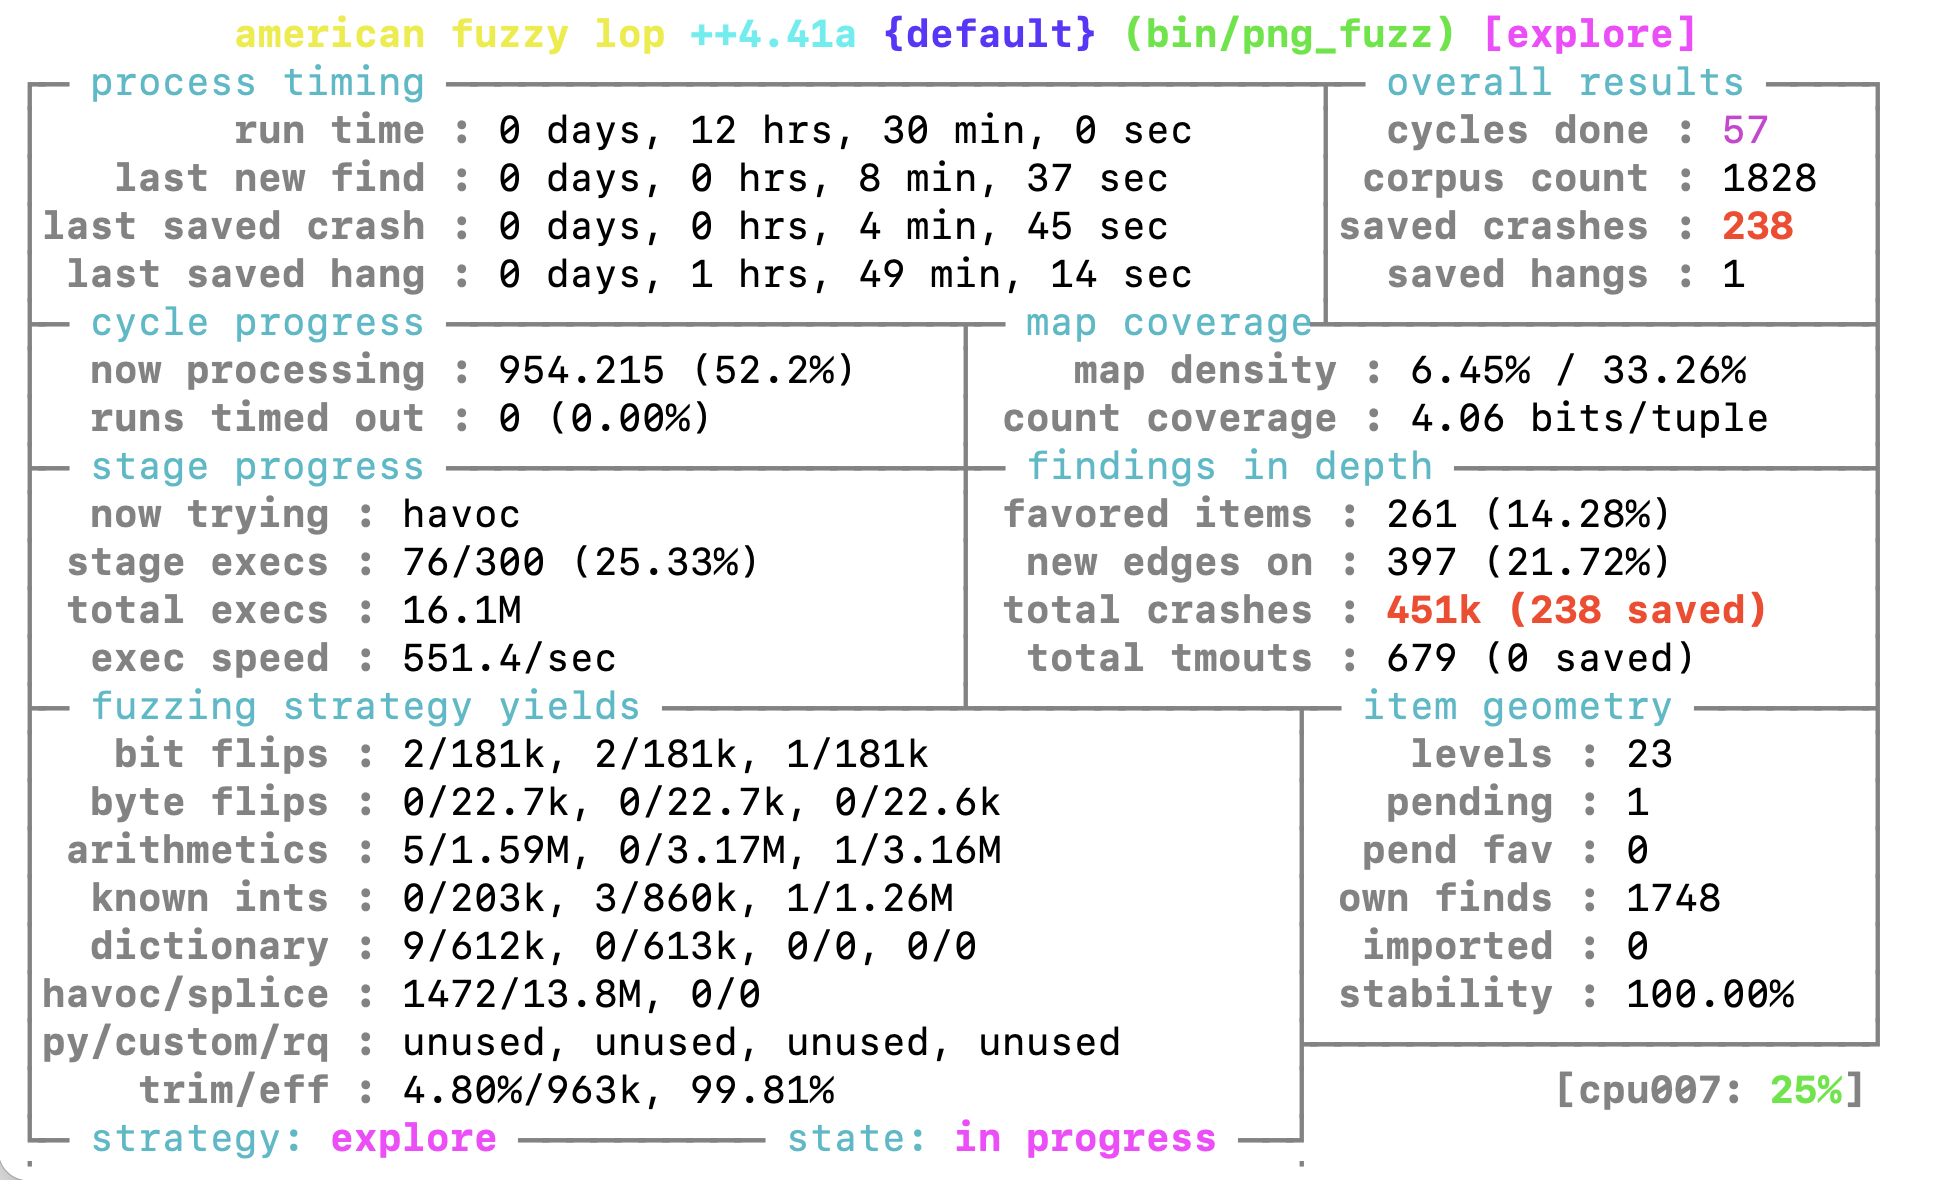
\includegraphics[width=1\linewidth]{figures/AFL_status_fork.png}
    \caption{}
    \label{fig:status_fork}
\end{subfigure}
\begin{subfigure}{0.48\textwidth}
    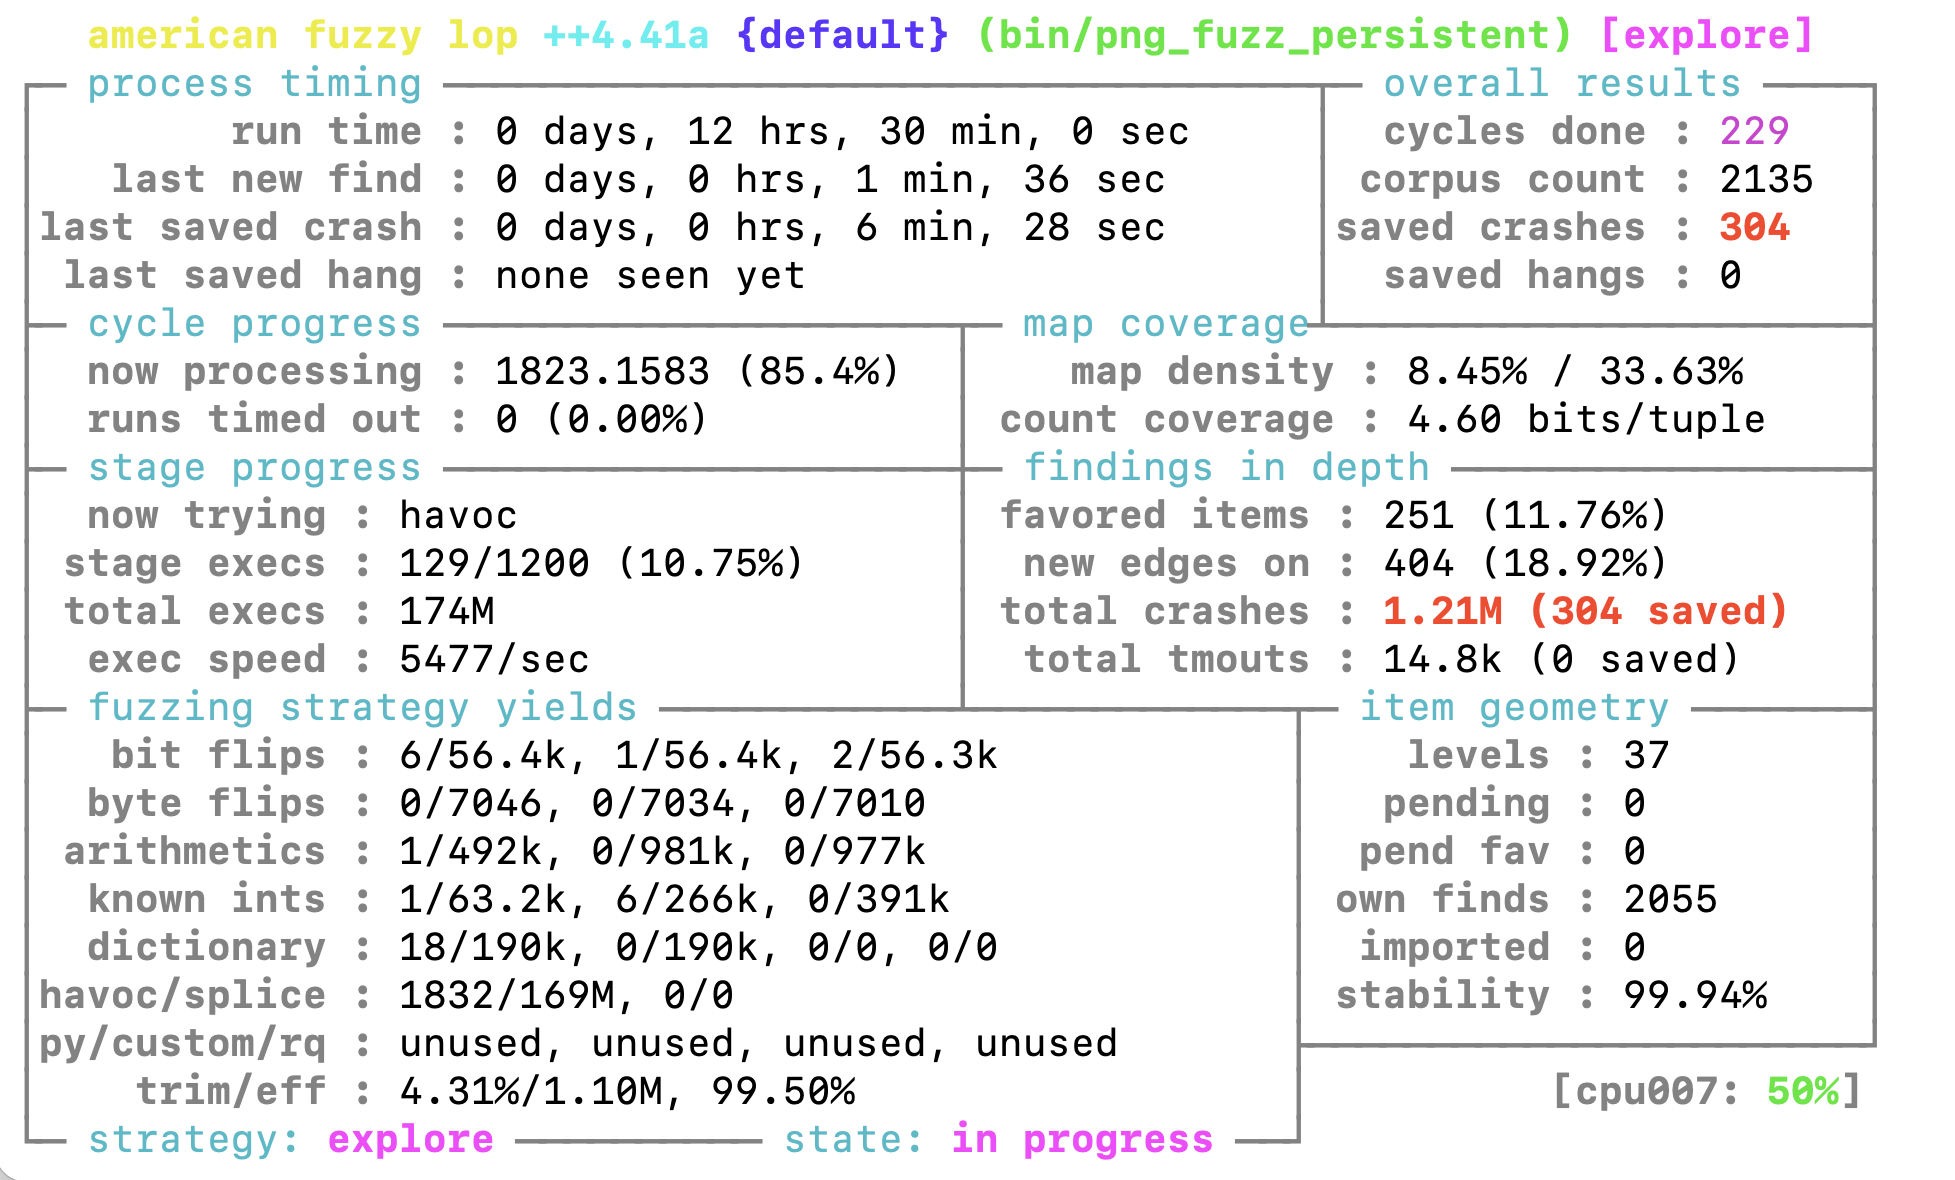
\includegraphics[width=1\linewidth]{figures/AFL_status_persistent.png}
    \caption{}
    \label{fig:status_persistent}
\end{subfigure}
\begin{subfigure}{0.48\textwidth}
    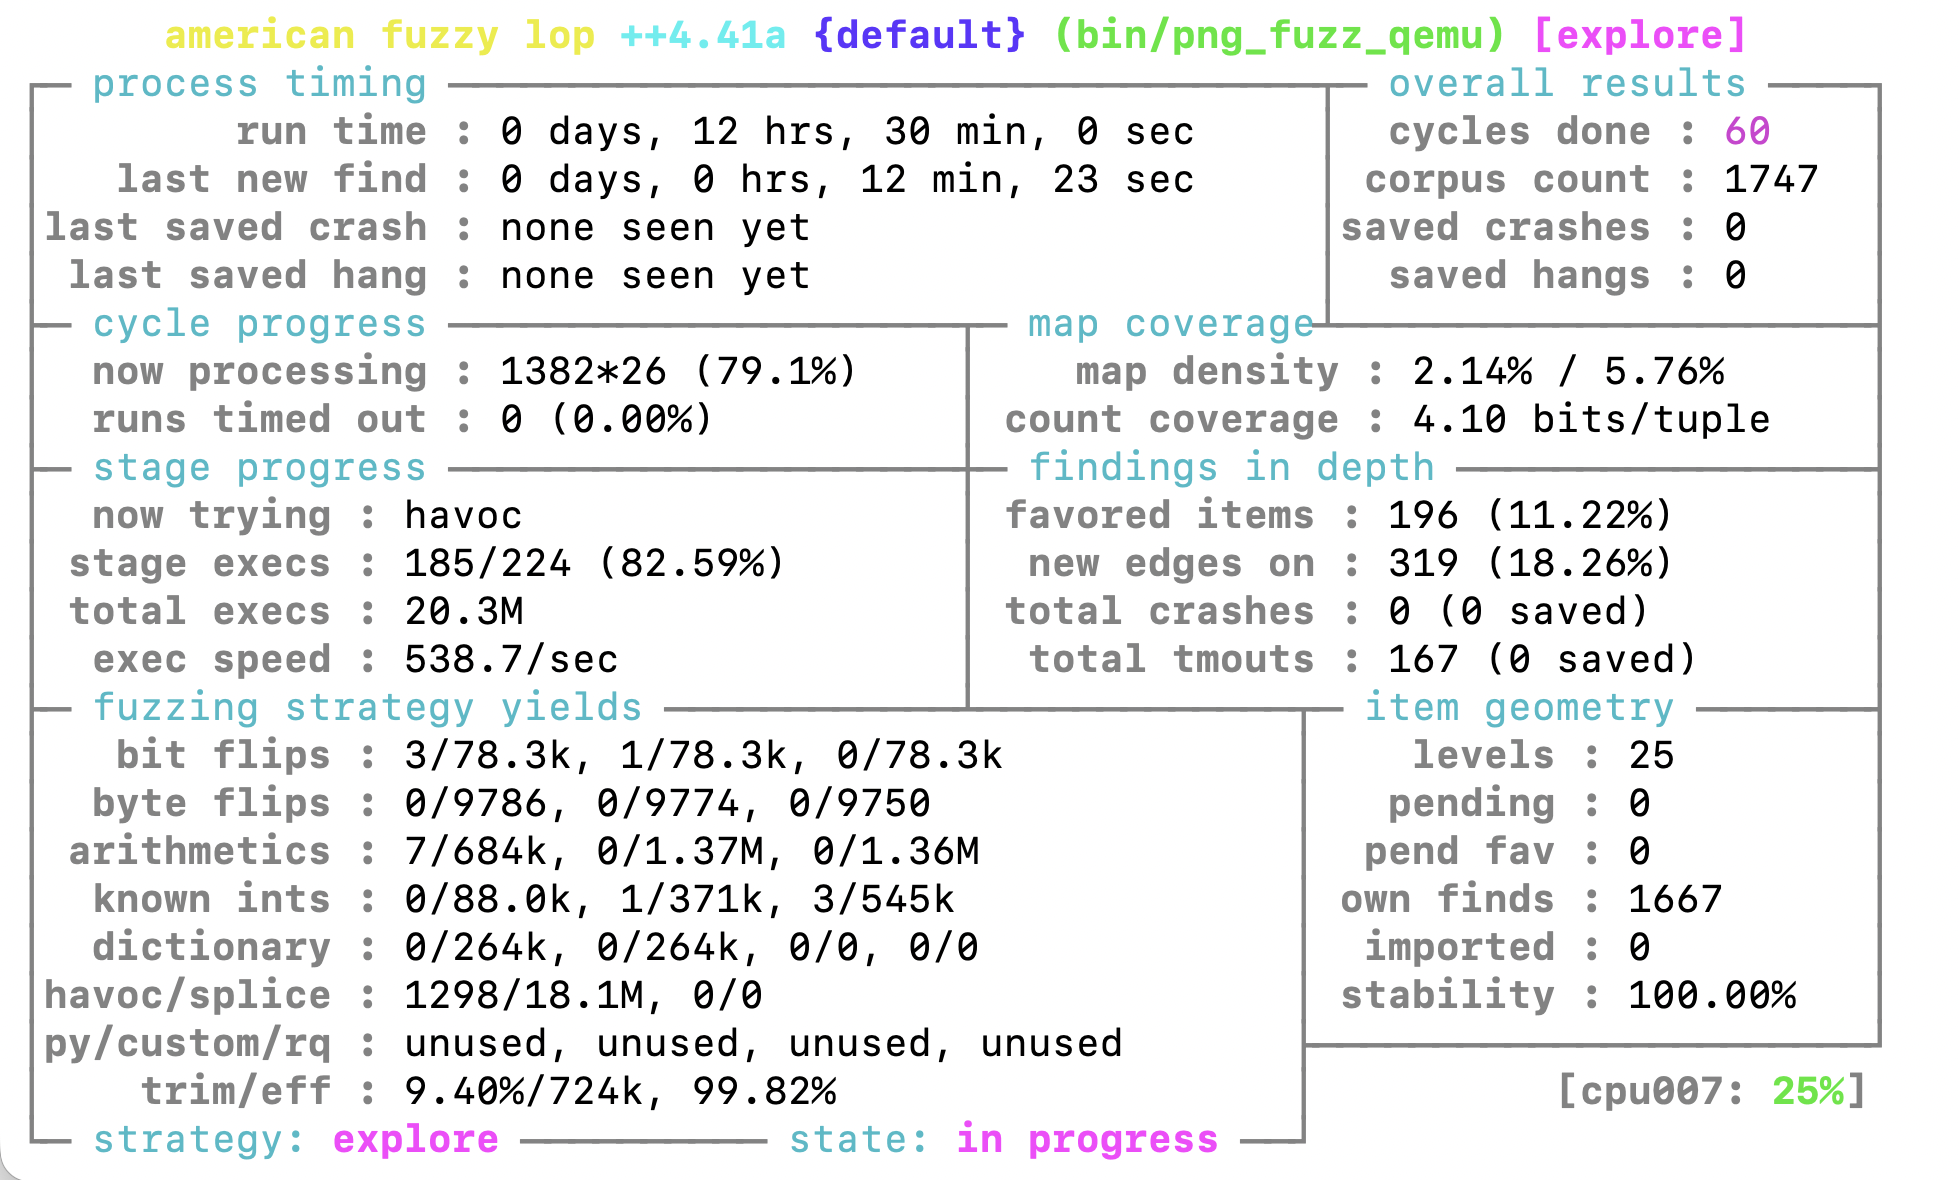
\includegraphics[width=1\linewidth]{figures/AFL_status_qemu.png}
    \caption{}
    \label{fig:status_qemu}
\end{subfigure}
    \caption{AFL++ status screen for the campaign of (a) and (b) the instrumented libpng library, with respectively the persistent was disabled and enabled, (c) the un-instrumented binary (qemu mode). All the campaign durations were 12 h 30 min. All three campaigns have been run simultaneously the same machine on three different CPU, so they were all subject to the same system conditions and are therefore directly comparable in terms of performance.}
    
\end{figure}
%======================================================
\newpage
\section{Fuzzing Campaign Results}
\subsection{For ASan and fork mode}
\setcounter{figure}{0}
\begin{figure}[h!]
\centering
\begin{subfigure}{0.75\textwidth}
    
\includegraphics[width=\textwidth]{figures/plot_output/edges}
    \caption{}
    \label{fig:fork_edges}
\end{subfigure}
\begin{subfigure}{0.75\textwidth}
    
\includegraphics[width=\textwidth]{figures/plot_output/exec_speed}
    \caption{}
    \label{fig:fork_exec_speed}
\end{subfigure}
\begin{subfigure}{0.75\textwidth}
    
\includegraphics[width=\textwidth]{figures/plot_output/high_freq}
    \caption{}
    \label{fig:fork_high_freq}
\end{subfigure}
\begin{subfigure}{0.75\textwidth}
    
\includegraphics[width=\textwidth]{figures/plot_output/low_freq}
    \caption{}
    \label{fig:fork_low_freq}
\end{subfigure}
\caption{Afl-plot data analysis of the campaign for the instrumented binary, with fork mode, for different metrics : (a) the number of edges, (b) the execution per second, (c) and (d) time evolution of different elements. The two gaps in the execution per second have been produced by the accidental sleep mode of the computer.}
\label{fig:plot_data_fork}
\end{figure}
%======================================================
\newpage
\subsection{ASan with Persistent Mode}

\begin{figure}[h!]
\centering
\begin{subfigure}{0.75\textwidth}
    
\includegraphics[width=\textwidth]{figures/plot_output_persistent/edges}
    \caption{}
    \label{fig:persistent_edges}
\end{subfigure}
\begin{subfigure}{0.75\textwidth}
    
\includegraphics[width=\textwidth]{figures/plot_output_persistent/exec_speed}
    \caption{}
    \label{fig:persistent_exec_speed}
\end{subfigure}
\begin{subfigure}{0.75\textwidth}
    
\includegraphics[width=\textwidth]{figures/plot_output_persistent/high_freq}
    \caption{}
    \label{fig:persistent_high_freq}
\end{subfigure}
\begin{subfigure}{0.75\textwidth}
    
\includegraphics[width=\textwidth]{figures/plot_output_persistent/low_freq}
    \caption{}
    \label{fig:persistent_low_freq}
\end{subfigure}
        
\caption{Afl-plot data analysis of the campaign for the instrumented binary, with persistent mode, for different metrics : (a) the number of edges, (b) the execution per second, (c) and (d) time evolution of different elements. The two gaps in the execution per second have been produced by the accidental sleep mode of the computer.}
\label{fig:plot_data_persistent}
\end{figure}

%======================================================
\newpage
\subsection{Qemu Mode}
\begin{figure}[h!]
\centering
\begin{subfigure}{0.75\textwidth}
    
\includegraphics[width=\textwidth]{figures/plot_output_qemu/edges}
    \caption{}
    \label{fig:qemu_edges}
\end{subfigure}
\begin{subfigure}{0.75\textwidth}
    
\includegraphics[width=\textwidth]{figures/plot_output_qemu/exec_speed}
    \caption{}
    \label{fig:qemu_exec_speed}
\end{subfigure}
\begin{subfigure}{0.75\textwidth}
    
\includegraphics[width=\textwidth]{figures/plot_output_qemu/high_freq}
    \caption{}
    \label{fig:qemu_high_freq}
\end{subfigure}
\begin{subfigure}{0.75\textwidth}
    
\includegraphics[width=\textwidth]{figures/plot_output_qemu/low_freq}
    \caption{}
    \label{fig:qemu_low_freq}
\end{subfigure}
        
\caption{Afl-plot data analysis of the campaign for the un-instrumented binary (qemu mode), for different metrics : (a) the number of edges, (b) the execution per second, (c) and (d) time evolution of different elements. The two gaps in the execution per second have been produced by the accidental sleep mode of the computer.}
\label{fig:plot_data_qemu}
\end{figure}
\newpage
\section{Q7 Campaigns}
\label{app:q7-evidence}
\setcounter{figure}{0}

Table~\ref{tab:qemu-comparison} compares the campaigns at the 30-minute mark. Appendix Figures~\ref{fig:instr-status} to~\ref{fig:qemu-execspeed} contain the supporting AFL++ status screens and \texttt{afl-plot} graphs.

\begin{table}[h!]
\centering
\small
\begin{tabular}{lcc}
\hline
Metric & Instrumented & QEMU mode \\
\hline
Wall-clock time & 1800 sec & 1800 sec \\
Exec speed & 313.8 exec/s & 295.7 exec/s \\
Corpus count & 1073 & 1080 \\
Edges found & 3158 & 3648 \\
Overall map density & 30.73\% & 5.57\% \\
Saved crashes & 71 & 0 \\
Total crashes & 2152 & 0 \\
Cycles done & 0 & 0 \\
Stability & 100.00\% & 100.00\% \\
\hline
\end{tabular}
\caption{Comparison between the source-instrumented campaign and the QEMU-mode campaign after 30 minutes.}
\label{tab:qemu-comparison}
\end{table}


\begin{figure}[h!]
\centering
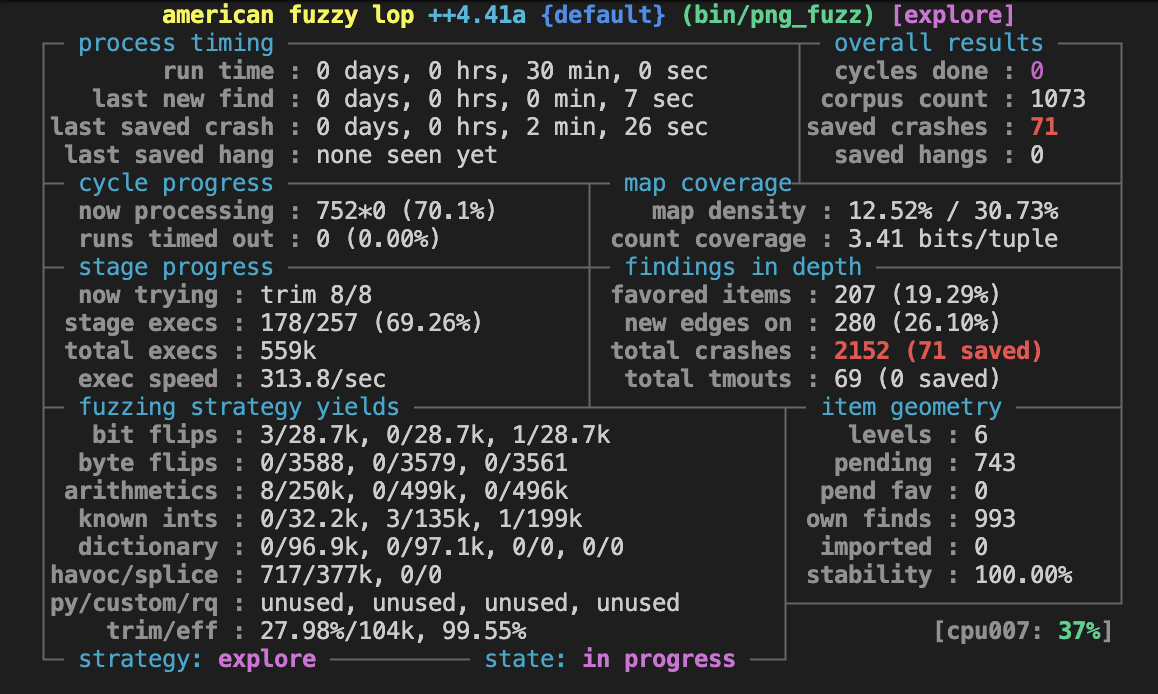
\includegraphics[width=0.95\textwidth]{figures/q7_instrumented_status.png}
\caption{AFL++ status screen for the source-instrumented campaign after 30 minutes.}
\label{fig:instr-status}
\end{figure}

\begin{figure}[h!]
\centering
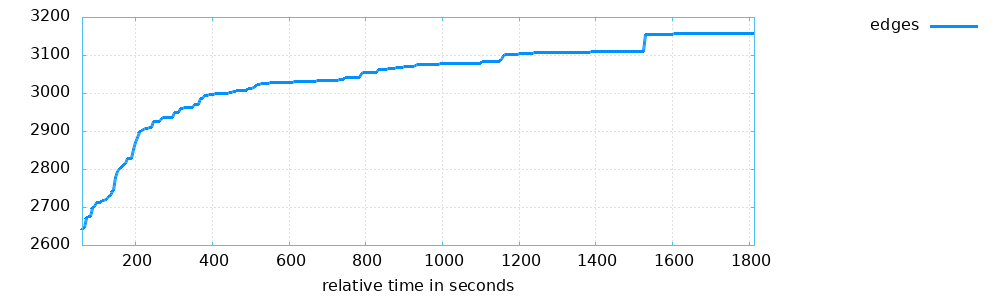
\includegraphics[width=0.95\textwidth]{figures/q7_instrumented_edges.png}
\caption{afl-plot edges graph for the source-instrumented campaign.}
\label{fig:instr-edges}
\end{figure}

\begin{figure}[h!]
\centering
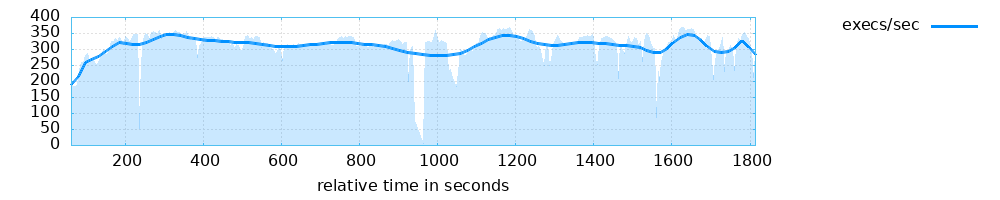
\includegraphics[width=0.95\textwidth]{figures/q7_instrumented_exec_speed.png}
\caption{afl-plot execution speed graph for the source-instrumented campaign.}
\label{fig:instr-execspeed}
\end{figure}

\begin{figure}[h!]
\centering
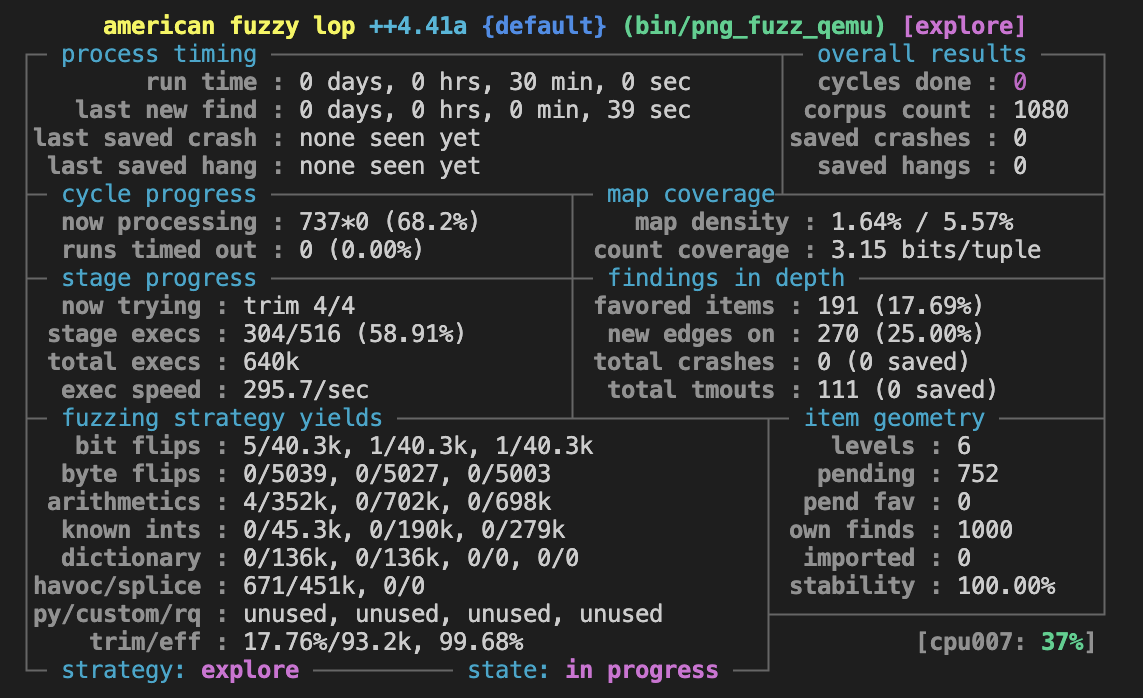
\includegraphics[width=0.95\textwidth]{figures/q7_qemu_status.png}
\caption{AFL++ status screen for the QEMU-mode campaign after 30 minutes.}
\label{fig:qemu-status}
\end{figure}

\begin{figure}[h!]
\centering
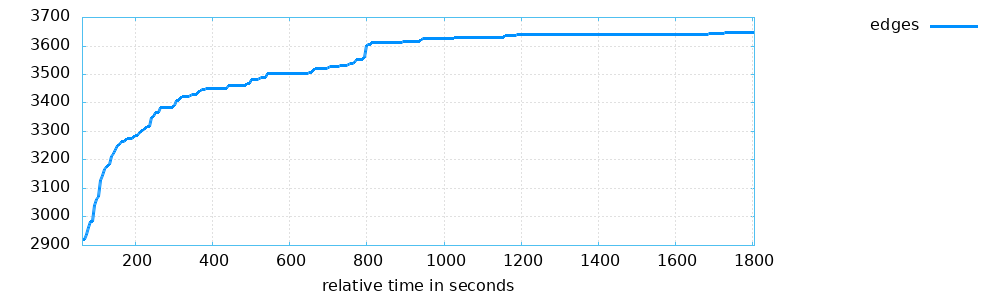
\includegraphics[width=0.95\textwidth]{figures/q7_qemu_edges.png}
\caption{afl-plot edges graph for the QEMU-mode campaign.}
\label{fig:qemu-edges}
\end{figure}

\begin{figure}[h!]
\centering
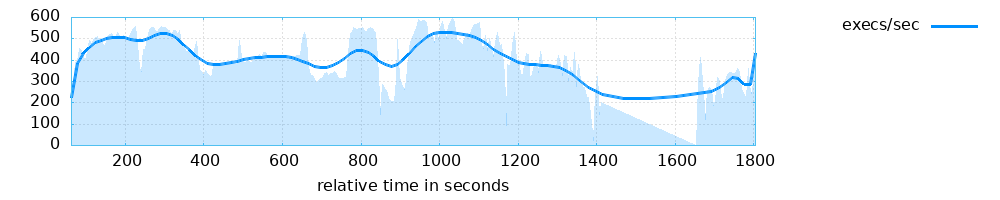
\includegraphics[width=0.95\textwidth]{figures/q7_qemu_exec_speed.png}
\caption{afl-plot execution speed graph for the QEMU-mode campaign.}
\label{fig:qemu-execspeed}
\end{figure}

\end{document}







